%**************************************************************************************
% License:
% CC BY-NC-SA 4.0 (http://creativecommons.org/licenses/by-nc-sa/4.0/)
%**************************************************************************************

\documentclass[notes]{beamer}

\mode<presentation> {

\usetheme{Madrid}

% Burnt orange
\definecolor{burntorange}{rgb}{0.8, 0.33, 0.0}
\colorlet{beamer@blendedblue}{burntorange}
% Pale yellow
\definecolor{paleyellow}{rgb}{1.0, 1.0, 0.953}
\setbeamercolor{background canvas}{bg=paleyellow}
% Secondary and tertiary palett
\setbeamercolor*{palette secondary}{use=structure,fg=white,bg=burntorange!80!black}
\setbeamercolor*{palette tertiary}{use=structure,fg=white,bg=burntorange!60!black}

% To remove the footer line in all slides uncomment this line
%\setbeamertemplate{footline}
% To replace the footer line in all slides with a simple slide count uncomment this line
%\setbeamertemplate{footline}[page number]

% To remove the navigation symbols from the bottom of all slides uncomment this line
%\setbeamertemplate{navigation symbols}{}
}

\usepackage{amsmath}
\usepackage{bm}
\usepackage{breqn}
\usepackage{graphicx} % for figures
\usepackage{subcaption} % for subplots 
\usepackage[labelsep=space,tableposition=top]{caption}
\renewcommand{\figurename}{Fig.} 
\usepackage{cleveref}
\usepackage{caption,subcaption}% http://ctan.org/pkg/{caption,subcaption}
\usepackage{booktabs} % Allows the use of \toprule, \midrule and \bottomrule in tables

%----------------------------------------------------------------------------------------
%	TITLE PAGE
%----------------------------------------------------------------------------------------
% The short title appears at the bottom of every slide, the full title is only on the title page
\title[CE394M: Intro to FEM]{CE394M Advanced Analysis in Geotechnical Engineering: FEM} 
\author{Krishna Kumar} % name
\institute[UT Austin] % institution 
{
University of Texas at Austin \\
\medskip
\textit{
  \url{krishnak@utexas.edu}} % Your email address
}
\date{\today} % Date, can be changed to a custom date

\begin{document}

\begin{frame}
\titlepage % title page as the first slide
\end{frame}

\begin{frame}
 % Table of contents slide, comment this block out to remove it
 \frametitle{Overview}
 % Throughout your presentation, if you choose to use \section{} and \subsection{} 
 % commands, these %will automatically be printed on this slide as an overview 
 \tableofcontents
\end{frame}

%----------------------------------------------------------------------------------------
% slides
%----------------------------------------------------------------------------------------

%------------------------------------------------
\section{Introduction to the Finite Element Analysis}
%------------------------------------------------
\begin{frame}
\frametitle{Finite Element Analysis}
 \noindent
\fboxsep=0pt
\noindent
\begin{minipage}[t]{0.42\linewidth}
	\begin{figure}
		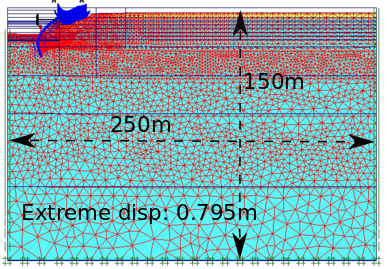
\includegraphics[width=0.95\textwidth]{figs/fea-geotech-mesh.png}
		\caption{FE Mesh}
	\end{figure}
\end{minipage}%
\hfill
\begin{minipage}[t]{0.56\linewidth}
	\begin{figure}
		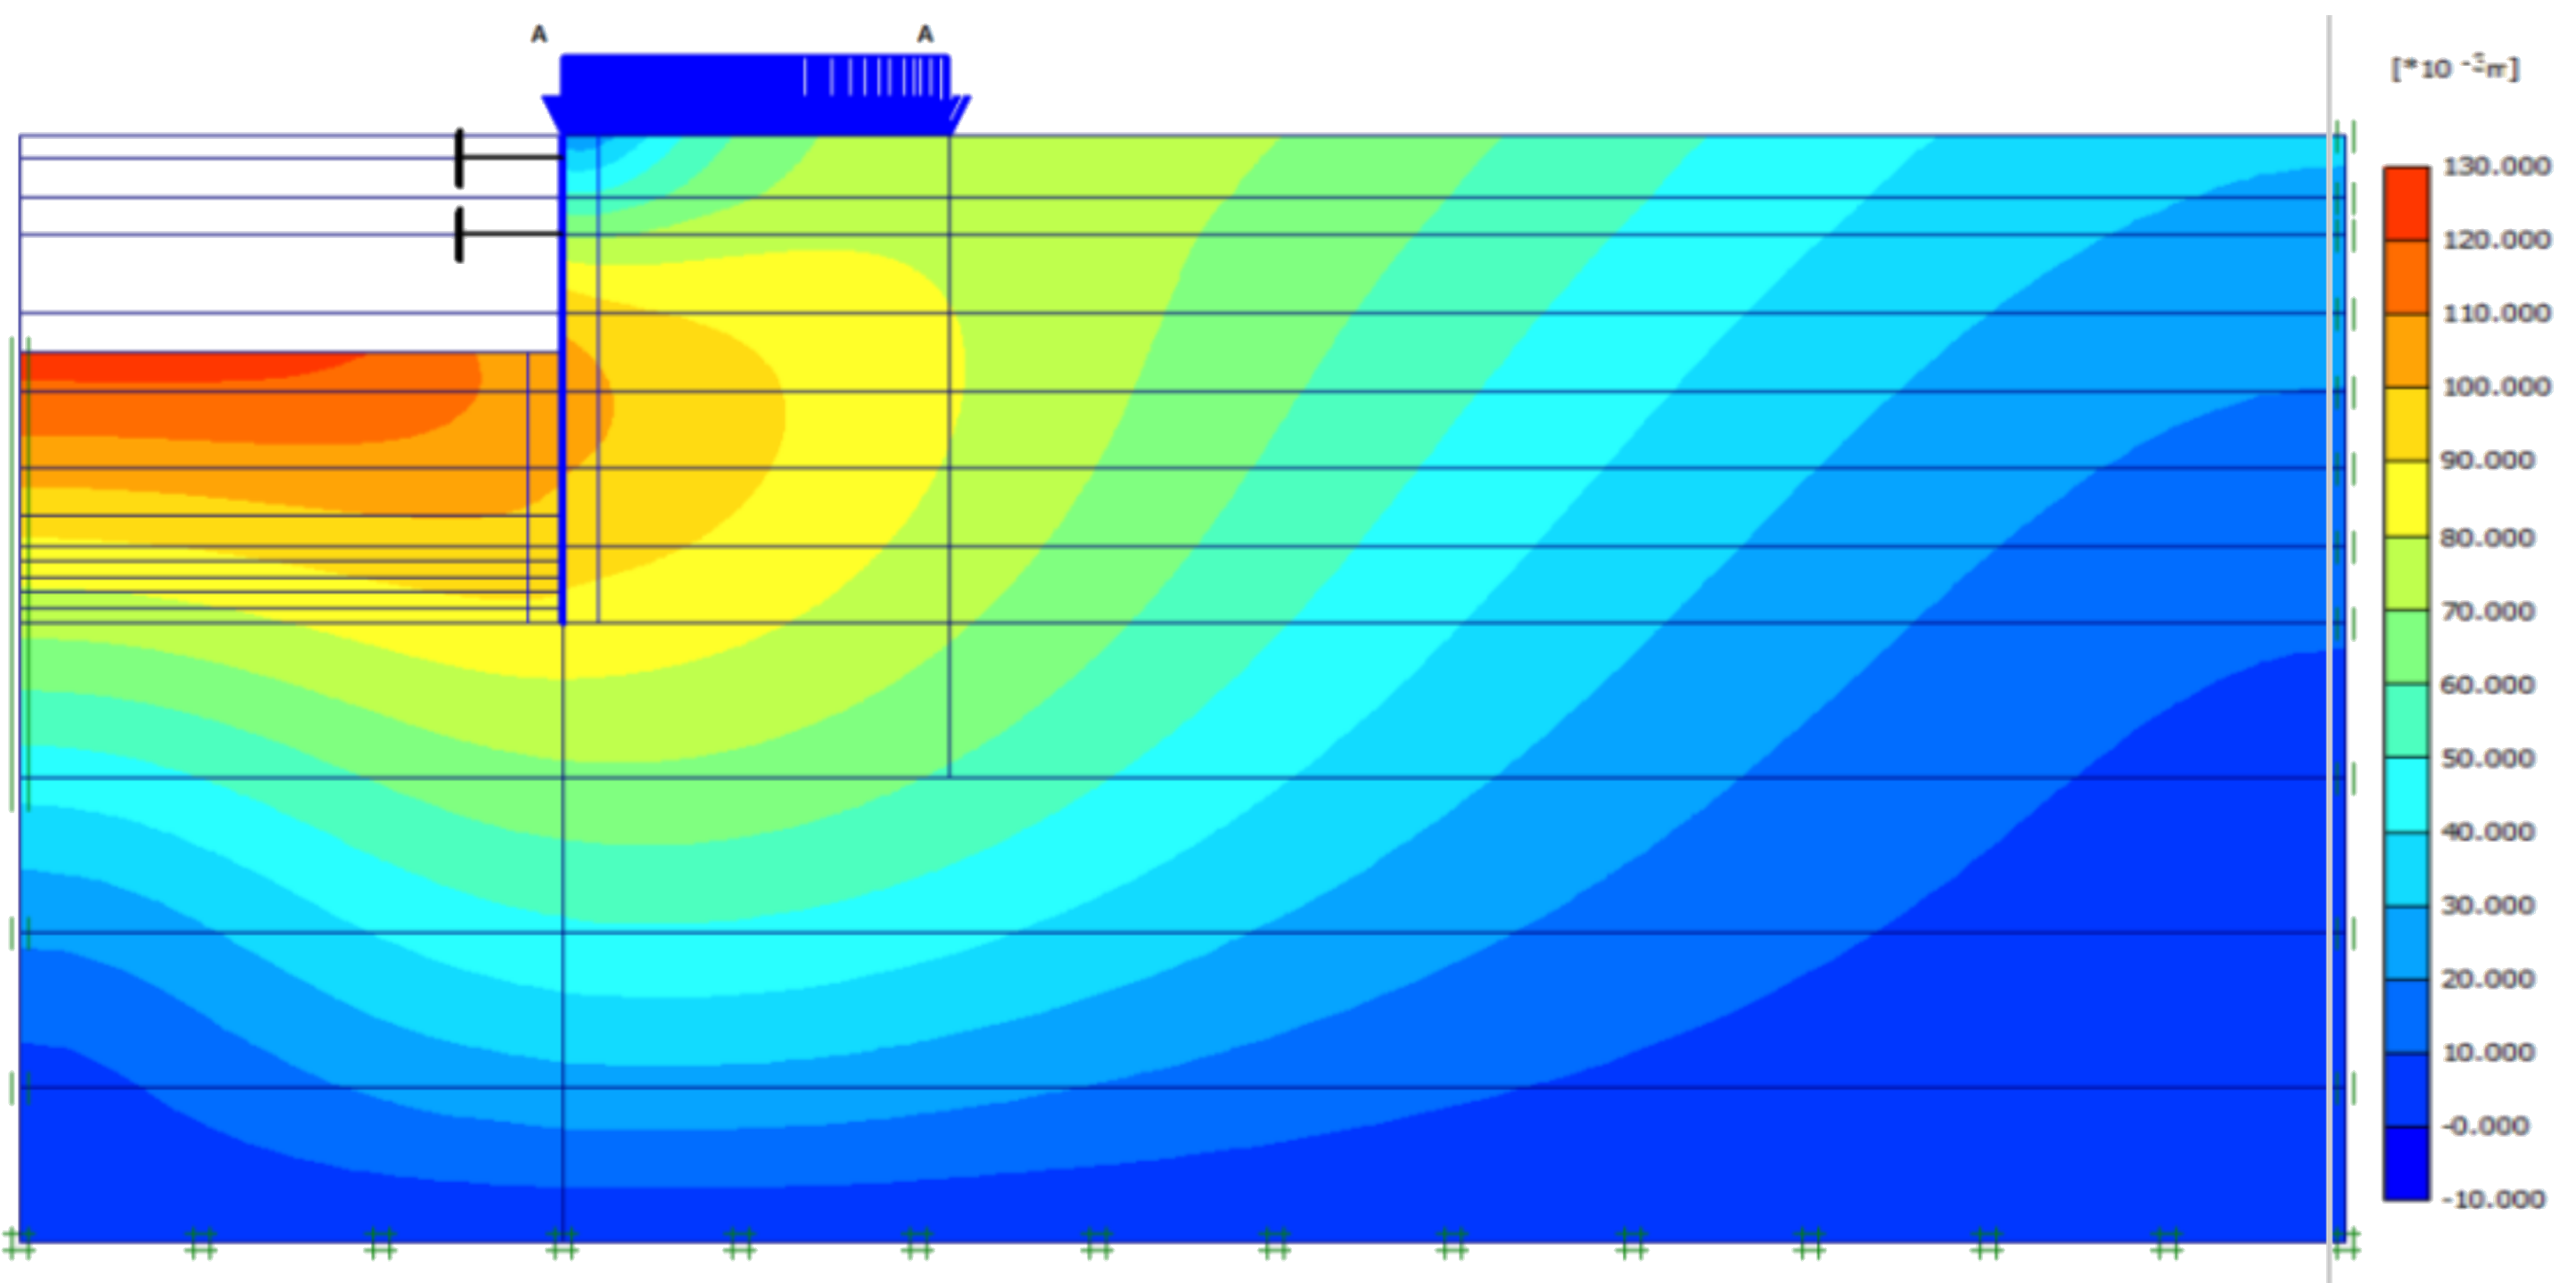
\includegraphics[width=\textwidth]{figs/fea-geotech.png}
		\caption{Displacement profile}
	\end{figure}
\end{minipage}
\centering
Singapore Nicoll highway excavation FE analysis
\end{frame}


%------------------------------------------------
\begin{frame}
\frametitle{Finite Element Approximations}
\mode<beamer>{
FE approximation of	$u$, which is a dependent variable in a PDE. 

\begin{figure}[ht]
	\centering
	\begin{subfigure}[b]{0.5\linewidth}
		\centering
		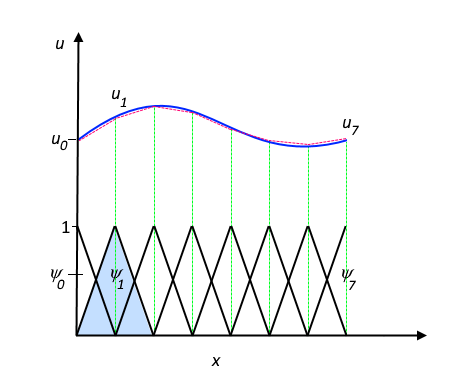
\includegraphics[width=0.8\textwidth]{figs/discretisation2.png}
	\end{subfigure}%
	\begin{subfigure}[b]{0.5\linewidth}
		\centering
		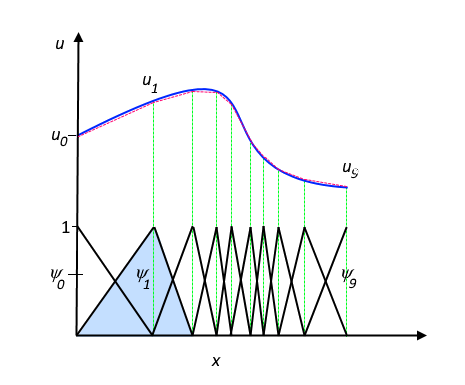
\includegraphics[width=0.8\textwidth]{figs/discretisation1.png}
	\end{subfigure}
	\caption*{FE basis functions}
\end{figure}
The function $u$ can be approximated by a function $u_h$ using linear combinations 
of basis functions according to the following expressions:
\begin{equation*}
u \approx u_h \quad u_h = \sum_{i} u_i \psi_i
\end{equation*}
}
\mode<handout>{
\vspace{5cm}
}
\end{frame}

\note{Geotechnical problems are usually expressed in terms of partial differential equations (PDEs), and for most problems, these PDEs cannot be solved with analytical methods. Instead, an approximation of the equations needs to be constructed, typically based upon different types of discretizations. These discretization methods approximate the PDEs with numerical model equations, which can be solved using numerical methods. The solution to the numerical model equations are, in turn, an approximation of the real solution to the PDEs. The finite element method (FEM) is used to compute such approximations.}
	
\note{Take, for example, a function $u$ that may be the dependent variable in a PDE (i.e., temperature, electric potential, pressure, etc.) The function u can be approximated by a function uh using linear combinations of basis functions according to the following expressions: 

\begin{equation*}
u \approx u_h \quad u_h = \sum_{i} u_i \psi_i
\end{equation*}

Here, $\psi_i$ denotes the basis functions and $u_i$ denotes the coefficients of the functions that approximate u with uh. The figure below illustrates this principle for a 1D problem. $u$ could, for instance, represent the temperature along the length ($x$) of a rod that is nonuniformly heated. Here, the linear basis functions have a value of 1 at their respective nodes and 0 at other nodes. In this case, there are seven elements along the portion of the x-axis, where the function u is defined (i.e., the length of the rod).}

\note{One of the benefits of using the finite element method is that it offers great freedom in the selection of discretization, both in the elements that may be used to discretize space and the basis functions. In the figure above, for example, the elements are uniformly distributed over the x-axis, although this does not have to be the case. Smaller elements in a region where the gradient of u is large could also have been applied.\\

Both of these figures show that the selected linear basis functions include very limited support (nonzero only over a narrow interval) and overlap along the x-axis. Depending on the problem at hand, other functions may be chosen instead of linear functions.\\

\url{https://www.comsol.com/multiphysics/finite-element-method}
}

\end{document} 
